\documentclass[10pt]{article}

\usepackage{mathtools}
\DeclarePairedDelimiter\ceil{\lceil}{\rceil}
\DeclarePairedDelimiter\floor{\lfloor}{\rfloor}


\usepackage{graphicx}
\graphicspath{{img/}}
\usepackage{amsmath}
\usepackage[margin=1.0in]{geometry}
\usepackage{hyperref}
\hypersetup{
	colorlinks=true,
	linkcolor=blue
}


\begin{document}

\title{\vspace{-2.0cm}Pacemaker Project Report}
\author{By: Neeraj Gandhi, Ramneet Kaur, Abhijeet Singh, Nikhil Shenoy}
\date{\today}

\maketitle

\section{Model Descriptions}
	In all the templates described below, x is a global clock that was declared in the “Descriptions” part of the model.

	\subsection{Heart}

		\begin{figure}[h]
			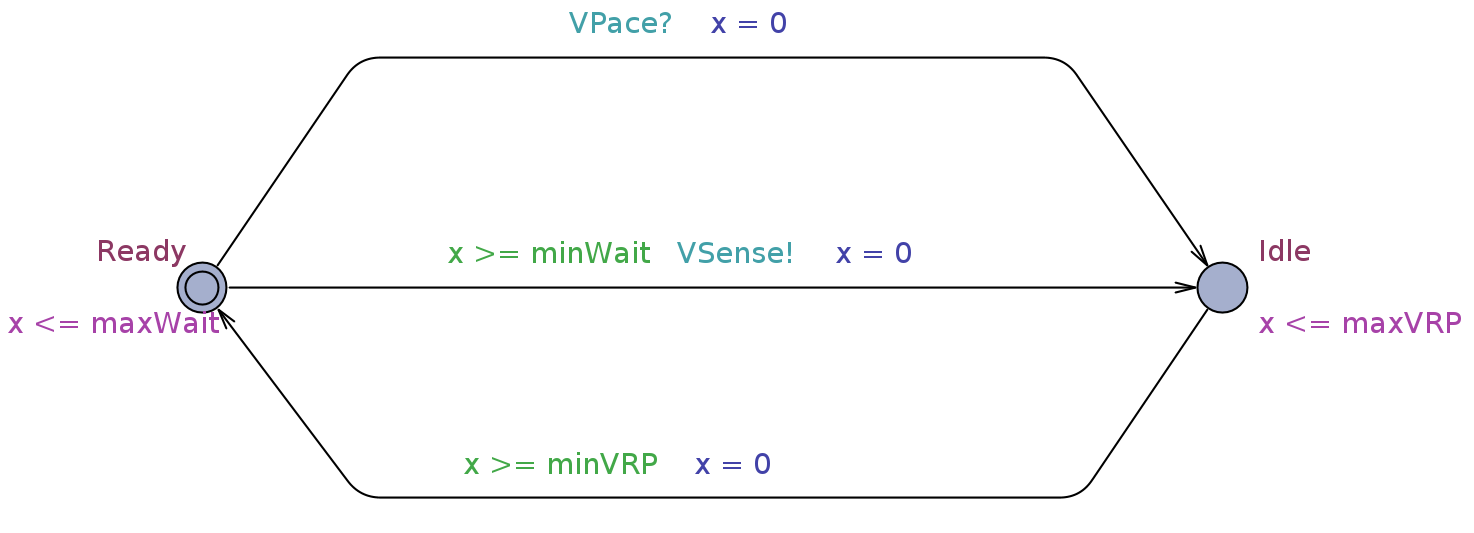
\includegraphics[scale=.35]{heart_model.jpg}
			\label{heart_model}
			\centering
			\caption{The Heart Model}
		\end{figure}

The Heart starts in the Ready state. It can either beat naturally (when it sends VSense!) or it can beat as a result of a simulated signal that the pacemaker sends (hence the synchronization with VPace?). The values for minWait and maxWait were selected based on estimations of what seemed reasonable, but they can be changed if other values are more appropriate.

	\subsection{Ventricle}
		\begin{figure}[h]
			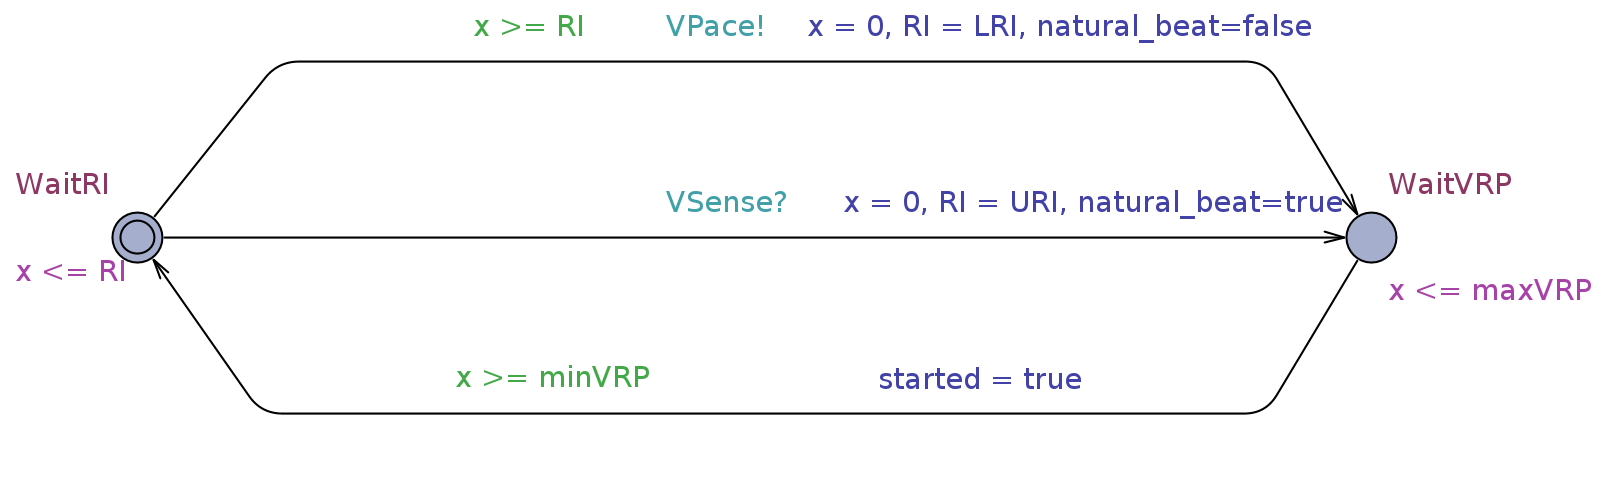
\includegraphics[scale=.4]{ventricle_model.jpg}
			\label{ventricle_model}
			\centering
			\caption{The Ventricle Model}
		\end{figure}

The Ventricle starts in the WaitRI state. Here, it waits to sense the occurrence of a natural heartbeat within a certain time frame, and if the time bound is exceeded it sends a stimulus to the heart. The Ventricle then moves into the WaitVRP state, which is a period during which no signals can be received. Once the VRP has elapsed, the Ventricle will return to the WaitRI state and wait for Sense signals. If this is the first cycle, a boolean called “started” will be set to true.

We have implemented hysteresis pacing in this model. That is, the pacemaker only sends a simulated beat when the natural beating period has surpassed HRI; after this, RI is set to LRI. The pacemaker will not cease simulated beating until the period of the patient’s heartrate is less than or equal to LRI, after which RI is reset to HRI.

The URI value is used to determine if the heart is beating too fast. At this point, there is nothing that the pacemaker can do, but it can set an alarm. This functionality is provided by the PostWaitPreSense and Sensed states. These synchronize the alarm with the Observer.

	\subsection{Observer}
		\begin{figure}[h]
			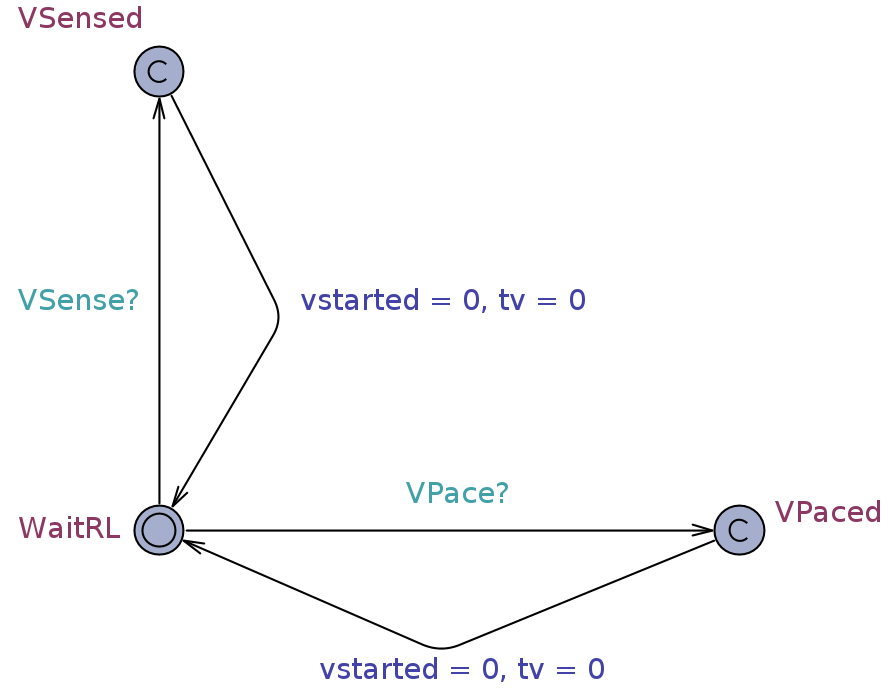
\includegraphics[scale=.4]{observer_model.jpg}
			\label{observer_model}
			\centering
			\caption{The Observer Model}
		\end{figure}

The Observer is used to model the external monitor of the interaction between the pacemaker and the heart. The Observer simply waits for a sensed heartbeat or a simulated heartbeat, changes states, and then changes states back. In the implementation, these state transitions would likely be logged so that if a doctor or someone else wanted to assess the health of the heart they could use the frequency of simulated heartbeats as an assessment parameter.

There is an alarm that will set the alarmSet variable if the natural beating frequency is greater than the maximum expected beating frequency (URI). We note that currently, the alarmSet variable is not triggering anything, but in the real implementation, the alarmSet variable will cause a notification to be sent to the doctor/patient.


\section{Query Descriptions}


	\subsection{A[] not deadlock}
		This is the standard deadlock query. This query makes sure that our system does not get stuck in a particular state and stop progressing.


	\subsection{A[] (Ventricle.x $<$ VRP \&\& Ventricle.started) imply (Ventricle.WaitVRP $||$ Ventricle.PostWaitPreSense $||$ Ventricle.Sensed)}

	If the system has started, the pacemaker will always be waiting for the ventricle refractory period to expire prior to doing anything else.

	\subsection{A[] ((Ventricle.WaitRI \&\& Ventricle.started \&\& !Ventricle.natural\_beat) imply Ventricle.x $<=$ Ventricle.LRI)}

	It will always be the case that if a simulated beat occurs, then the pacemaker will wait for a natural beat for the length of the LRI before continuing to pace.

	\subsection{A[] ((Ventricle.WaitRI \&\& Ventricle.started \&\& Ventricle.natural\_beat) imply Ventricle.x $<=$ Ventricle.HRI)}

It will always be the case that if the heart has been beating normally, then the pacemaker will wait until the heart rate is less than hysteresis rate before intervening.

	\subsection{A[] ((Ventricle.WaitRI \&\& Ventricle.started)) imply Ventricle.x $>=$ VRP}

	It is always the case that if the system has started and is currently waiting, the ventricle refractory period of the previous beat-cycle is complete.

	\subsection{A[] (Ventricle.x $<$ Ventricle.URI \&\& Ventricle.Sensed imply Observer.alarmSet $==$ true)}

	If the heart is beating faster than the upper rate limit, then an alarm will be set on the monitor. 

\section{References}

	\begin{enumerate}
		\item PACEMAKER System Specification, Copyright 2007 Boston Scientific, January 3, 2007.
		\item Pacemaker Timing Cycles-F13-F17-v3.pdf, CIS 441/541: Embedded Systems for CPS/IoT, Fall 2017 by Prof. Insup Lee, Department of Computer and Information Science, School of Engineering and Applied Science, University of Pennsylvania.
		\item Kirk, M. \textit{Basic principles of pacing: Chapter 1}. \url{http://www.blackwellpublishing.com/content/BPL\_Images/Content\_store/Sample\_chapter/9780727915665/Chow%20Sample%20Chap%201.pdf}
	\end{enumerate}


	
\end{document}









